\documentclass[11pt]{article}
\usepackage{multicol}
\setlength{\columnseprule}{1pt} % separation line between columns
\setlength{\parindent}{0pt} % paragraph indentation

\usepackage[top=2cm, bottom=2cm, left=2cm, right=2cm]{geometry}
\usepackage[T1]{fontenc}
\usepackage[utf8]{inputenc}
\usepackage[francais]{babel}
\usepackage{textcomp}

\usepackage{hyperref}
\hypersetup{
	colorlinks=true,       	% false: boxed links; true: colored links
	linkcolor=black,          	% color of internal links
	urlcolor=blue,           	% color of external links
	citecolor=blue
}

\usepackage{dashrule}
\usepackage{wrapfig}
\usepackage{graphicx}
\usepackage{enumitem}
\usepackage{wrapfig}
\usepackage{cancel} % diagonal strikeout
\usepackage[margin=1cm]{caption}
\setdescription{leftmargin=1cm,labelindent=0.5cm}

\usepackage{amsmath}
\usepackage{amssymb}
\usepackage{amsfonts}

\newcommand\mathd[0]{\mathrm{d}} 

\usepackage{blindtext}

% Colors
\usepackage[usenames,dvipsnames]{xcolor}
\definecolor{session_bg}{RGB}{25,25,25}
\definecolor{grey2}{rgb}{0.3,0.3,0.3}
\definecolor{dkgreen}{rgb}{0,0.6,0}
\definecolor{gray}{rgb}{0.5,0.5,0.5}
\definecolor{mauve}{rgb}{0.58,0,0.82}
\definecolor{blue}{rgb}{0,0,0.7}

% Colored frame
\usepackage{framed}
\definecolor{shadecolor}{rgb}{0.96,0.96,0.96}
\definecolor{TFFrameColor}{rgb}{0.96,0.96,0.96}
\definecolor{TFTitleColor}{rgb}{0.00,0.00,0.00}

% Redefine leftbar environment
\newlength{\leftbarwidth}
\setlength{\leftbarwidth}{1pt}
\newlength{\leftbarsep}
\setlength{\leftbarsep}{10pt}

\newcommand*{\leftbarcolorcmd}{\color{leftbarcolor}} % as a command to be more flexible
\colorlet{leftbarcolor}{gray}

\renewenvironment{leftbar}{%
    \def\FrameCommand{{\leftbarcolorcmd{\vrule width \leftbarwidth\relax\hspace {\leftbarsep}}}}%
    \MakeFramed {\advance \hsize -\width \FrameRestore }%
}{%
    \endMakeFramed
}

\usepackage{listings}
\lstloadlanguages{C,sh}
\lstdefinestyle{session}{
	numbers=left,	
	tabsize=4,
	frame=single, % cadre autour du code
	basicstyle=\small\ttfamily\color{white},
	numberstyle=\scriptsize\ttfamily,
	backgroundcolor=\color{session_bg},
	showstringspaces=false,
	keywordstyle=\color{OliveGreen},
	stringstyle=\color{BrickRed},
	commentstyle=\color{grey2}\it,
	stepnumber=1
}
\lstdefinestyle{C}{
    language=[ANSI]C,
	basicstyle=\scriptsize,
	numbers=left,                   % where to put the line-numbers
  	numberstyle=\tiny\color{gray},
	commentstyle=\color{dkgreen},
	frame=single,                   % adds a frame around the code
 	rulecolor=\color{black},
	emph={},
	emphstyle=\color{mauve},
	morekeywords={},
	keywordstyle={\color{blue}},
	showstringspaces=false
}

% Title page
\title{Création d'une interface graphique et interactive \\ pour jeux de rôles papier}
\author{
	Damien Martel \\ \href{mailto:damien.martel@edue.esiee.fr}{damien.martel@edu.esiee.fr} \and
	Bertrand Le Mée \\ \href{mailto:bertrand.lemee@edu.esiee.fr}{bertrand.lemee@edu.esiee.fr} \and
	Vincent Lindivat \\ \href{mailto:vincent.lindivat@edu.esiee.fr}{vincent.lindivat@edu.esiee.fr} \and
	Frédéric Nguyen \\ \href{mailto:frederic.nguyen@edu.esiee.fr}{frederic.nguyen@edu.esiee.fr}
}
\date{\today}

\begin{document}
\maketitle
\newpage
\hfill
\newpage
\tableofcontents
\newpage

\section{Introduction}

Le jeu de rôles est un jeu qui regroupe plusieurs joueurs dans la même salle qui incarnent chacun un personnage pour jouer ensemble. Ils sont guidé par un Maître Jeu qui orchestre le bon déroulement des sessions. Le jeu est accompagné de beaucoup de matériels tels que les dés, le plateau et les jetons. Cependant, un inconvénient se fait ressentir. Il faut que toutes les personnes se trouvent dans la même pièce. Il n'est donc pas toujours facile pour les joueurs de se retrouver, particulièrement lorsqu'ils se situent loin géographiquement. \\

Ayant ces éléments à l'esprit, nous avons développé une interface graphique qui permet d'organiser des parties de jeu de rôles à distance sur réseau. Nous avons fait attention à ne pas dépayser les utilisateurs en conservant au mieux l'atmosphère du jeu plateau habituel. \\

Ce projet est une opportunité pour nous de découvrir le travail de développement en équipe sur un projet de plus grande envergure que ce que nous avons réalisé jusqu'à maintenant.	

\section{Méthode agile SCRUM}

A l'occasion de ce projet, nous avons pu découvrir la méthode de développement
 agile SCRUM  et dans le même mouvement, appliquer cette méthode à la réalisation de notre projet.\\
 
Dans le cadre SCRUM, les trois entités suivantes se rassemblent autour du projet :

\begin{description}
	\item[Product Owner] \hfill \\
		Il définit les fonctionnalités du projet et décide de valider ou non les résultats. Il met en place les dates à respecter. Le Product Owner établit aussi le \textit{Backlog} avec le Scrum Master et l'équipe, mais il peut modifier un \textit{Sprint} si besoin.
	\item[Scrum Master] \hfill \\
		Il s'occupe de l'équipe de développement en veillant à ce la méthode SCRUM soit bien appliquée. Il conseille son équipe et s'assure qu'elle progresse correctement. Il gère aussi les relations extérieures, particulièrement avec le Product Owner.
	\item[Equipe de développement] \hfill \\
		Généralement constituée de 5 à 10 personnes, l'équipe regroupe tout type de rôle. Une équipe travaille sur un \textit{Sprint} et est libre de s'organiser d'elle-même.
\end{description}

La progression du projet est basée sur un \textbf{Backlog}, faite par le Product Owner, le Scrum Master et l'équipe, qui est une liste ordonnée par priorité et complexité de temps de tâches à réaliser. Les priorités sont choisies par le Product Owner et peuvent être revues selon le courant des événements. \\

Durant le projet, le temps est divisé en séquence ayant une durée moyenne de 2 semaines, ces séquences sont appelées \textbf{Sprint}. Avant chaque Sprint, l'équipe choisit dans le Backlog l'ensemble des tâches qu'elle compte pouvoir réaliser. \\

Quotidiennement, une réunion d'une quinzaine de minutes \textbf{debout} se fait dans l'équipe afin de faire le point sur ce qui a été fait le jour précédent et ce qui va être fait le jour de la réunion. Lorsqu'un Sprint est terminé, le Product Owner, le Scrum Master et l'équipe se rassemble pendant 30 minutes pour faire le point ce qui a marché et ce qui n'a pas marché afin de mieux préparer et agir lors du prochain Sprint. \\

N'étant qu'une équipe de 4 et le projet ne durant que 2 mois, nous avons dû réadapter la méthode. Nous nous sommes convenus de faire des Sprints de une semaine et travailler de façon très souple pendant les temps de travail.

\section{SFML}
\section{SFML}

Au début de notre projet, nous avions pensé à utiliser une bibliothèque graphique spécialisée dans la réalisation de jeu, SFML (\textit{Simple and Fast Multimedia Library}).\\

Cette bibliothèque nous aurait permis de réaliser facilement des animations et toute sorte d'effet graphique. 
Cependant, en utilisant SFML, de mauvaises réactions ont été constatées, notamment au niveau de l'affichage de la fenetre SFML.
Après plusieurs difficultés à faire cohabiter Qt et SFML, nous avons, au bout de deux semaines, nous avons décidé de réaliser l'application exclusivement avec Qt. Pour cela, nous avons dû repenser entièrement le système de carte déjà réalisé avec SFML.

\section{Manuel d'utilisation}

Cette application débute avec une boîte de dialogue qui laisse le choix entre deux rôles : Maître Jeu (MJ) ou Joueur. Si MJ est choisi, l'application se met en tant que serveur pour accueillir les joueurs. Si joueur est choisi, un assistant ce connexion apparaît pour choisir à quel serveur se connecter. \\

L'interface qui se présente comporte un Chat, un gestionnaire de tours et le lanceur de dés. Le Chat contient la liste des utilisateurs et permet aux joueurs et au MJ de communique. De plus, le chat possède des commandes qui s'introduisent par un /. Les commandes implémentées sont :

\begin{description}
	\item[/help] \hfill \\
		Affiche l'ensemble des autres commandes disponibles du chat avec les indications d'utilisation.
	\item[/nickname <pseudo>] \hfill \\
		Modifie le pseudo par celui qui suit la commande.
	\item[/roll <nombre de dés>d<valeur max du dé>] \hfill \\
		Roule un nombre de fois voulu du dé choisi. Peu s'utiliser en chuchotement.
	\item[/whisper <utilisateur> <message>] \hfill \\
		Envoie un message privé au joueur indiqué.
\end{description}

\begin{figure}[h!]
	\centering
	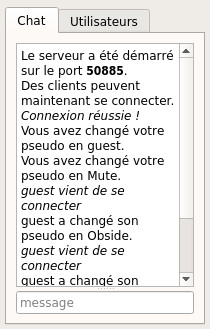
\includegraphics[scale=0.5]{img/chat_mj.jpg}
	\hspace{10 mm}
	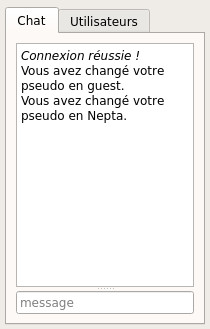
\includegraphics[scale=0.5]{img/chat_player.jpg}
	\caption{Chat MJ (à gauche) et chat Joueur (à droite)}
\end{figure}

\section{Conclusion}

\end{document}